\begin{figure}
  \centering
  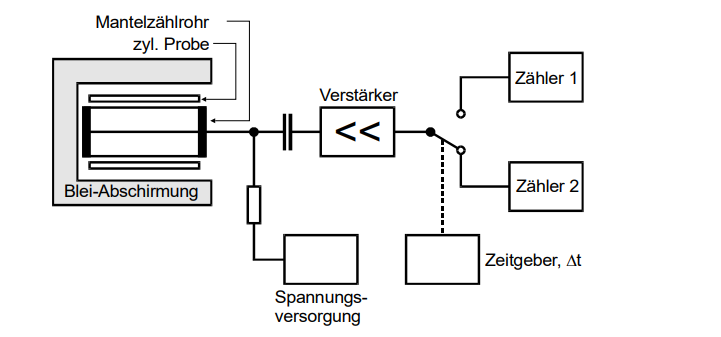
\includegraphics[width=0.8\textwidth]{bilder/Schematische Darstellung des Versuchsaufbaus.png}
  \caption{Apparatur als schematische Darstellung \cite{skript}.}
  \label{fig:aufbau}
\end{figure}
Der Aufbau besteht hauptsächlich aus einem Geiger-Müller-Zählrohr, eingepackt in einem Abschirmblock aus Blei. Dies hat den Nutzen das Zählrohr von externen 
radioaktiven Strahlungen abzuschirmen. Die Dort gemessenen Impulse werden von einem Verstärker aufgegriffen und zu einem sogenannten Zählwerk weitergeleitet. 
Das Zählwerk selbst beinhaltet zwei Anzeigevorrichtungen. 
Im Aufbau auch zu erkennen \ref{fig:aufbau} ist eine Spannungsversorgung für den Geiger-Müller-Zähler sowie den Verstärker und das Zählwerk. 
Der Zeitgeber schaltete automatisch zwischen Zwei Zählern nach einer Zeit $\Delta t$ um.

